% Modelo de relatório no estilo artigo em duas colunas
\documentclass[twocolumn]{article}
\usepackage[utf8]{inputenc}
\usepackage{amsmath}
\usepackage{subcaption}
\usepackage{mathtools}
\usepackage{graphicx}
\usepackage{color}
\usepackage{authblk}
\usepackage{lmodern}
% \usepackage[colorlinks,citecolor=black,urlcolor=black,bookmarks=false,hypertexnames=true]{hyperref}
\usepackage{geometry}
\usepackage{pdfpages}
\usepackage{fancyhdr}
\usepackage[utf8]{inputenc}

\usepackage[sorting=none,style=numeric]{biblatex}
\addbibresource{refs.bib}
\usepackage[justification=centering]{caption}
\usepackage{makecell}
\usepackage{booktabs}
\usepackage{hhline}
\usepackage{amsmath}
\usepackage{amssymb}
\usepackage{soul}
\usepackage{gensymb}
\usepackage{listings}

\setlength\parindent{0pt}


\newcommand{\myname}{Nishant Aswani}
\newcommand{\mynetid}{nsa325}
\newcommand{\myemail}{nsa325@nyu.edu}
\newcommand{\myhwtype}{Lab }
\newcommand{\myhwnum}{2}
\newcommand{\mycoursenumber}{ENGR-UH 3511}
\newcommand{\myclassname}{Computer Organization and Architecture}
\newcommand{\myassignmenttitle}{MIPS Assembly, Recursion and the SPIM simulator}
\newcommand{\myinstructor}{Cristoforos Vasilatos}

\newcommand{\cc}[1]{\texttt{#1}}

\lstset{
  basicstyle=\ttfamily,
  escapeinside=||
}

% Tamanho das margens:
% \geometry{
% 	a4paper,
% 	total={170mm,257mm},
% 	left=30mm,
% 	top=20mm,
% }
%%%%%%%%%%%%%%%%%%%%%%%%%%%%%%%%%%%%%%%%%
% Bibliografia estilo ABNT. Se não tiver instalado, comente a linha abaixo.
% \usepackage[alf, abnt-etal-list=0, abnt-emphasize=bf,abnt-last-names=bibtex, abnt-etal-text=it, abnt-etal-cite=2]{abntex2cite}
%%%%%%%%%%%%%%%%%%%%%%%%%%%%%%%%%%%%%%%%%

% Dados de identificação
\title{\myassignmenttitle}
\author{\myname, \myemail}
\affil{\myclassname (\mycoursenumber), Instructor \myinstructor}
\date{}

\begin{document}
%%%%%%%%%%%%%%%%%%%%%%%%%%%%%%%%%%%%%%%%%%%%%%%% COVER PAGE %%%%%%%%%%%%%%%%%%%%%%%%%%%%%%%%%%%%%%%%%%%%%%%%%%%%
\onecolumn
\pagestyle{fancy}
\fancyhf{}
\renewcommand{\headrulewidth}{0pt}
\rhead{\textbf{Division of Engineering}}
\lhead{\textbf{NYU Abu Dhabi}}

\begin{center}
  
\includegraphics[scale=0.15]{etc/NYUAD-alt-logo.jpg}
\end{center}

{\vspace{2.5em}}

\begin{center}
    \Huge{\textbf{\mycoursenumber}}\\
    {\vspace{0.5em}}
    \Huge{\textbf{\myclassname}}
\end{center}

{\vspace{10em}}

\begin{center}
  \begin{tabular}{|rp{5.0cm}lll|}
    \hline
    &  &  &  & \\
    &  &  &  & \\
    \Large{\textbf{Name:}} & \Large{\myname}
    
    \  &  &  & \\
    \Large{\textbf{Net ID:}} & \Large{\mynetid}
    
    \  &  &  & \\
    \Large{\textbf{Assignment Title:}} & \Large{\myhwtype \myhwnum}
    
    \
    
    \  &  &  & \\
    \hline
  \end{tabular}
\end{center}

\

{\newpage}
%%%%%%%%%%%%%%%%%%%%%%%%%%%%%%%%%%%%%%%%%%%%%%%% COVER PAGE %%%%%%%%%%%%%%%%%%%%%%%%%%%%%%%%%%%%%%%%%%%%%%%%%%%%

\maketitle        

% Resumo de no máximo 200 palavras
% \begin{abstract}
% Este documento orienta a descrição das atividades práticas desenvolvidas em laboratório. São usados como exemplo conceitos da Aula 01 de Acionamentos Elétricos sobre partida direta de motor de indução trifásico. Nesta atividade, um motor é acionado com conexões estrela e triângulo a vazio. As correntes nominais e de partida são medidas com amperímetro analógico e comparadas entre si. Nota-se que, mesmo sem carga, as corrente em estrela são maiores. 
% \end{abstract}

\section{Introduction}

The MIPS architecture falls under the reduced instruction set computer (RISC) family of instruction set architectures (ISAs). During the 1980s and 1990s, the MIPS architecure was used for general computing. However, it has now been relinquished for use in embedded systems. MIPS is a 32-bit architecture, employing 32 registers, each 32 bits wide. Since current computers do not use a MIPS architecure, tools such as SPIM are used to simulate the MIPS architecure. The following lab uses the MIPS assembly to implement a matrix multiplier and a recursive exponent calculator.

\section{Methodology}

\subsection{2x2 Matrix Multiplier}

For the matrix multiplier, the traditional triple nested loop algorithm was modeled in MIPS assembly. 

\begin{verbatim}
for (int i=0; i<N; ++i)
    for (int j=0; j<N; ++j)
        for (int k=0; k<n; ++k)
            C[i][j] = A[i][k] + B[k][j]
\end{verbatim}

To begin with, the .data section was built, consisting of a result message, two input arrays, the predetermined matrix size, and an array initialization for the resulting array. 

\begin{verbatim}
.data
resultMessage: .asciiz "Resulting matrix [(0,0), (0,1), (1,0), (1,1)]: \n"
arr1: .word 2,-1,1,3    # first 2x2 array
arr2: .word 5,6,7,8     # second 2x2 array
matrixSize: .byte 2     # square matrix size
res: .word 0:4          # result aray
newline: .asciiz "\n"
\end{verbatim} 

Next, the main function was built, storing the base addresses of the arrays into registers for later use. The matrix size was also stored for easy use with loop counter limits. At the end, a jump tag was added to begin the nested loops.

\begin{verbatim}
.text
main:
  la $a1, arr1          # store base address of array 1 in register
  la $a2, arr2          # store base address of array 2 in register
  lb $a3, matrixSize    # store matrixSize into register
  la $t8, res           # store base address of result array in register
  j L1                  # jump to L1 (first loop)
\end{verbatim}

However, the caveat is that in MIPS assembly, the traditional multidimensional indexing is not available. \\

Hence, an algorithm must be devised to simulate this indexing within a flat array. \\

Given multidimensional indexing, the following methodology is used for matrix multiplication: 

\begin{equation}
    \begin{split}
        C_{0,0} & = A_{0,0}*B_{0,0} + A_{0,1}*B_{1,0} \\
        C_{0,1} & = A_{0,0}*B_{0,1} + A_{0,1}*B_{1,1} \\
        C_{1,0} & = A_{1,0}*B_{0,0} + A_{1,1}*B_{1,0} \\
        C_{1,1} & = A_{1,0}*B_{0,1} + A_{1,1}*B_{1,1} \\
    \end{split}
\end{equation}

In order to carry this out in a 1D array, a pattern was determined:

\begin{equation}
    \begin{split}
        C[0] & = A[0]B[0] + A[1]B[2] \\
        C[1] & = A[0]B[1] + A[1]B[3] \\
        C[2] & = A[2]B[0] + A[3]B[2] \\
        C[3] & = A[2]B[1] + A[3]B[3] \\
    \end{split}
\end{equation}

Examining the pattern, the following formula was derived: 

\begin{equation}
    \begin{split}
        C[2i+j] &= A[2i+k] + B[j+2k]
    \end{split}
\end{equation}

Combining this formula with the nested loop structure, the following MIPS assembly code was developed. Arriving at loop 1, the branch statement checks whether the "i counter" has hit the limit, which is the matrix size. If not, it organically moves onto the next loop, once again checking if the "j counter" has hit the limit. It then naturally moves into the third loop, which carries out the same check. 

\begin{verbatim}
L1:
  beq $t0, $a3, L1end   # if i = matrixSize then go to L1end
  
L2:
  beq $t1, $a3, L2end   # if j = matrixSize then go to L2end
  
L3:
  beq $t2, $a3, L3end   # if k = matrixSize then go to L3end
\end{verbatim}

Each of the checks, if met, take the program to their respective "ends." The end of the inner most loop (k-loop in C++ implementation), simply increments the j counter and loops to the top of loop 2 to check whether its condition has been meet. The end of loop 2 does a similar check, taking the program to the end of loop 1 if the branch statement is met. The end of loop 1 means that the nested loop has been fully carried out and it is time to print the result. 

\begin{verbatim}
L1end:
  j printInit
  
L2end:
  addi $t0, $t0, 1      # increment i counter by 1
  li $t1, 0             # reset j counter to 0
  j L1                  # jump to j loop
  
L3end:
  addi $t1, $t1, 1      # increment j counter by 1
  li $t2, 0             # reset k counter to 0
  j L2                  # jump to k loop
\end{verbatim}

The bulk of the work occurs within L3 (the kth loop), which can also be seen in the C++ implementation. \\

To reiterate, the branch statement checks whether the loop has hit the limit, so that it may increment the counter above it (j-counter). Then, the following "initializations" show the upcoming chunks.\\

The first chunk loads the address of $A[2i+k]$ , the second chunk loads the address of $B[j+2k]$, and the third chunk loads the addres of the result array at $C[2i+j]$.

\begin{verbatim}
L3:
  beq $t2, $a3, L3end   # if k = matrixSize then go to L3end

  li $t4, 0  		    # use $t4 to hold needed array 1 addresses
  li $t5, 0   		    # use $t5 to hold needed array 2 addresses
  li $t6, 0   		    # use $t6 to hold needed result array addresses
  li $t7, 0   		    # use $t7 to store result from loop
\end{verbatim}

To load $A[2i+k]$, the "i counter" must be multiplied by 2 using the shift left method. It is then added to the "k counter". It is important to note that (2i+k) must be multiplied by 4 to get correct address offset because the MIPS architecture assigns 4 bytes to an int. Once the offset is obtained, it is added to the base address of the first array to obtain the value inside. 

\begin{verbatim}
  # loading the value from array 1
  sll $t4, $t0, 1       # i*2
  add $t4, $t4, $t2     # 2i+k
  sll $t4, $t4, 2       # (2i+k)*4 to get offset
  add $t4, $t4, $a1     # address A[0] + (2i+k)*4
  lw  $t4, 0($t4)       # load A[2i+k] into $t4 
\end{verbatim}

Similarly, the value from the second array is obtained. 

\begin{verbatim}
  # loading the value from array 2
  sll $t5, $t2, 1       # k*2
  add $t5, $t5, $t1     # j+2k
  sll $t5, $t5, 2       # (j+2k)*4 to get offset
  add $t5, $t5, $a2     # address B[0] + (j+2k)*4
  lw  $t5, 0($t5)       # load B[j+2k] into $t5 register
\end{verbatim}

Finally, the address for where the value must be stored in the resulting array is obtained. 

\begin{verbatim}
  # loading the address for result
  sll $t6, $t0, 1       # i*2
  add $t6, $t6, $t1     # 2i+j
  sll $t6, $t6, 2       # (2i+j)*4 to get offset 
  add $t6, $t6, $t8     # address C[0] + (2i+j)*4
\end{verbatim}

Once all values are loaded, the multiplication between the value from the first array and second array is carried out and stored into a register.  

\begin{verbatim}
  # carry out multiplication A[i][k]*B[k][j]
  mul $t7, $t4, $t5
\end{verbatim}

However, this value cannot directly be stored into the resulting array, because it may overwrite the existing value written in that location, when it should be added to it. \\

This problem arises because this implementation in assembly breaks the dot product into two steps; if using a high-level language, the addition would be carried out in the same loop. 

\begin{verbatim}
  # add onto existing value to avoid overwrite
  lw  $t9, 0($t6)	# load existing value 
  add $t7, $t7, $t9	# add new value onto existing value
\end{verbatim}

Finally, the value is stored into the result array and the loop is brought back to the top for a branch check. 

\begin{verbatim}
  # save into result array at C[i][j]
  sw  $t7, 0($t6)	# save value into result array

  # conclude loop
  addi $t2, $t2, 1      # increment k counter by 1
  j L3                  # return to start of L3
\end{verbatim}

As mentioned earlier, once the outermost loop is completed, the program is sent to printing the resulting matrix. \\

A loop counter is set up with a branch comparison checking whether it has hit the limit, which is the size of the array. In each loop, the counter is offset by 4 bytes and added to the base address of the result array to point to the next value needed to be printed. Then built-in MIPS calls are used to print to screen.

\begin{verbatim}
printMatrix:
  beq $t3, $t9, exit    # if loop counter = matrixSize**2 then exit
  
  sll $t7, $t3, 2       # (counter)*4
  add $t7, $t7, $t8     # address C[0] + (counter)*4
  
  li  $v0,1             # code for print_int
  lw $a0, 0($t7)        # put result in $a0
  syscall               # print out the result
  
  li $v0, 4             # code for print_string
  la $a0, newline       # point $a0 to newline
  syscall               # print the result
  
  addi $t3, $t3, 1      # increment print loop counter
  j printMatrix         # loop back to beginning of printMatrix
\end{verbatim}

Once the print counter has hit the limit, it runs the exit label. 

\begin{verbatim}
exit:
  li $v0, 10            # code for exit
  syscall               # exit program
\end{verbatim}

\subsection{Recursive Power of 3}

A recursive implementation of the power of 3 problem takes advantage of the stack and jal instruction, which provides a return address to the next instruction. \\

To begin with, the .data section is set-up consisting of messages to display to the user and the exponent base being used, in this case 3. 

\begin{verbatim}
.data
promptMessage: .asciiz "Please input an integer: \n" 
resultMessage: .asciiz "The power of three is: "
base: .byte 3     	    # base value set to 3
newline: .asciiz "\n"	# newline
\end{verbatim}

The program begins by displaying a prompt message and taking in input for the n value, to which 3 is raised to. The n value is moved into the \$a1 register to follow convention.

\begin{verbatim}
.text
main: 
  li $v0,4                  # code for print_string
  la $a0,promptMessage      # point $a0 to result string
  syscall                   # print the result string 
  
  li $v0,5                  # code for read_int
  syscall                   # get int from user --> returned in $v0
  move $a1, $v0             # move user input to $a1
  lb $a2, base              # save base into register $a2
\end{verbatim}

Next, the program prepares for the recursive implementation. It first takes care of the base case, storing 1 into the return value register for when the recursive calls start returning. \\

The next instruction is a jump to the powerRec label. Here it is important to the note that the return address points to the print label. Hence, the final return address in the stack will point to this label. 

\begin{verbatim}
powerInit:
  li $v1, 1             # account for base case: when recursion ends multiply by 1
  jal powerRec          # jump to powerRec and store next instruction into $ra
  
print:
  li $v0,4              # code for print_string
  la $a0,resultMessage  # point $a0 to result string
  syscall               # print the result string 
\end{verbatim}

Looking at the powerRec label, the first instruction decreases the stack pointer value by 4 bytes. This is because the stack "grows" from bottom up. Hence, we must go "backwards" in memory to build up the stack. The return address is then stored into the stack. \\

In the initial case, the first return address to be stored is that of the print label. As the powerRec label is looped, the return address is actually of the instruction right after the jal instruction. \\

So, when "popping" occurs, the mul instruction will be called the designated number of times to multiply the stored value by 3. \\

\begin{verbatim}
powerRec: 
  addi $sp, $sp, -4     # decrement stack pointer by 4
  sw $ra, 0($sp)        # save return address to stack pointer

  beqz $a1, return      # if recursive counter equals 0 begin returning
  addi $a1, $a1, -1	    # decrement the value of recursive counter
  
  jal powerRec          # loop back to power function
  
  mul $v1, $v1, $a2     # multiply 3 by value in $v1 register during return
\end{verbatim}

Each time the powerRec loop occurs, the number of recursions (stored in \$a1) is decremented. Once it hits zero, the return label is called. \\

The return label simply looks into the stack and returns the address stored from top to bottom, then points a byte down in the stack. All of these returns, except the last one, are to the mul instruction seen above. The final return is to the print label shown earlier.

\begin{verbatim}
return:
  lw $ra, 0($sp)        # load the return address from the top 
  addi $sp, $sp, 4      # move the stack pointer "downward"
  jr $ra                # jump to the return address
\end{verbatim}

The print label simply carries out the conventional MIPS calls to print out the result message and the resulting value of $3^n$. 

\begin{verbatim}
print:
  li $v0,4              # code for print_string
  la $a0,resultMessage  # point $a0 to result string
  syscall               # print the result string 
  
  li  $v0,1             # code for print_int
  move $a0, $v1         # put result in $a0
  syscall               # print out the result
  
  li $v0, 4             # code for print_string
  la $a0, newline       # point $a0 to newline
  syscall               # print the result
  
  j exit
\end{verbatim}

Once printing is completed, there is a simple jump to the exit label, which terminates the program

\begin{verbatim}
exit:
  li $v0, 10            # code for exit
  syscall               # exit program
\end{verbatim}

\newpage

\section{Results}

\subsection{2x2 Matrix Multiplier}

Given the following matrix input: 

\begin{center}
  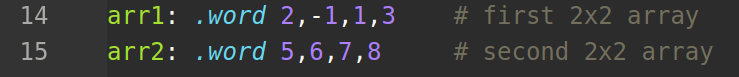
\includegraphics[scale=0.6]{Lab2-images/matmul2.png}
\end{center}

Running the program in SPIM results in: 

\begin{center}
  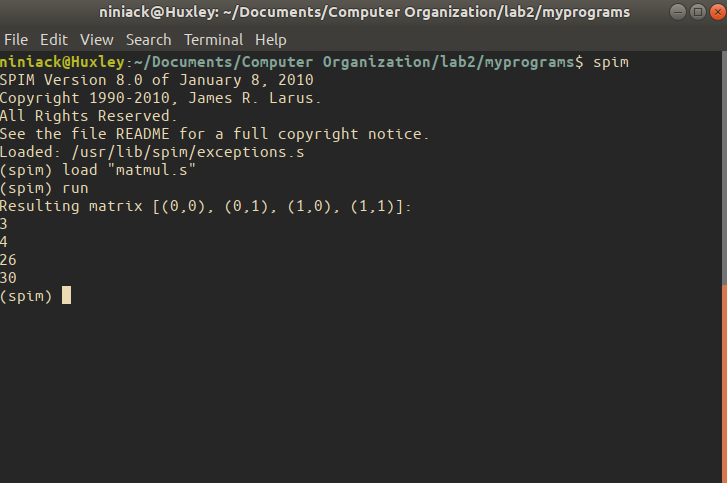
\includegraphics[scale=0.45]{Lab2-images/matmul.png}
\end{center}

The program is able to multiply square matrices beyond size 2 as well. However, some parameters and output messages have to be rewritten to make the output meaningful. \\

Overall, the results were successful, though printing the result was not convenient using MIPS. 

\newpage

\subsection{Recursive Power of 3}

Running the program with different inputs ($10\leq n<20$): 

\begin{center}
  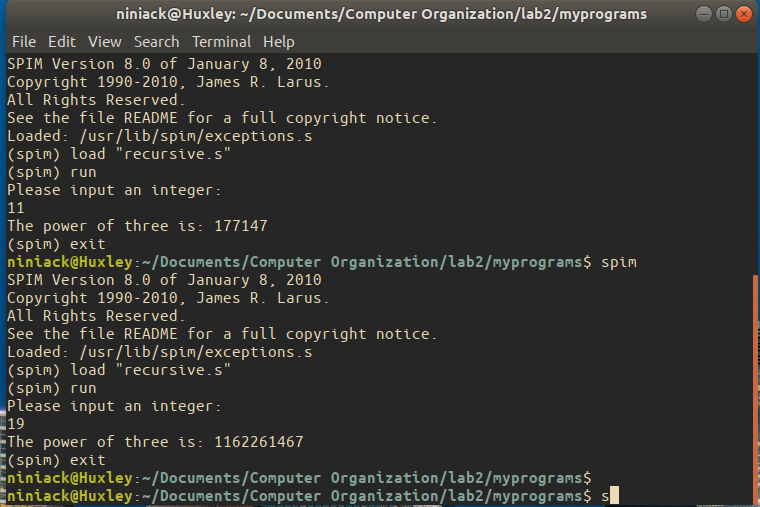
\includegraphics[scale=0.45]{Lab2-images/recursive.png}
\end{center}

The program is capable of calculating exponents of other bases as well. Once again, some parameters and output messages have to be rewritten to make the output meaningful. \\

Below is an example of using base 2. 

\begin{center}
  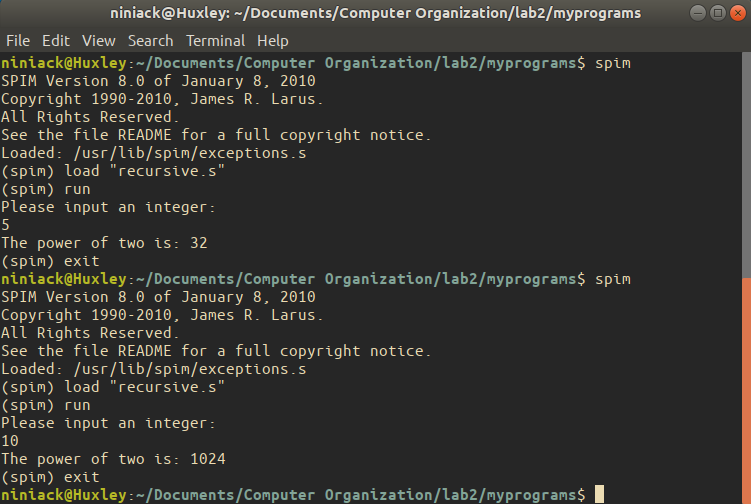
\includegraphics[scale=0.45]{Lab2-images/recursive2.png}
\end{center}






%%%%%%%%%%%%%%%%%%%%%%%%%%5
% BIBLIOGRAFIA 
% Estilo de bibliografia ABNT. Se não tiver instalado, mude para plain ou ieeetr

%\bibliographystyle{plain} % Inclua isso se não tiver ABNTEX instalado
% \begin{thebibliography}{refs}
% \bibitem{}
\printbibliography
% \end{thebibliography}
\end{document}